\documentclass[12pt]{article}
\usepackage[english]{babel}
\usepackage{cite}
\usepackage{amsmath}
%\usepackage[latin1]{inputenc}
%\usepackage[dvips]{graphics}
%\usepackage{graphicx}
%\usepackage{epsfig}
%\usepackage{latexsym}
\usepackage{amssymb}
%\usepackage[T1]{fontenc}
\usepackage{theorem}
\usepackage{algorithmicx}
\usepackage[ruled]{algorithm}
\usepackage{algpseudocode}

\usepackage{graphicx} % figuras
\usepackage{subfigure} % subfiguras


\usepackage[active]{srcltx}
%\numberwithin{equation}{section}
\renewcommand{\theequation}{\arabic{equation}}
\DeclareMathOperator{\e}{e} %La exponencial
\DeclareMathOperator{\sinhc}{sinhc}

\newcommand{\re}[1]{\textrm{#1}} %letra redondilla en f�rmulas matem�ticas
\newcommand{\norm}[1]{\left\Vert#1\right\Vert}
\newcommand{\RE}{\operatorname{Re}}
\newcommand{\IM}{\operatorname{Im}}


\newtheorem{Theorem}{\bf Theorem}[section]
\newtheorem{lemma}{\bf Lemma}%[section]
\newtheorem{definition}{\bf Definition}%[section]
\newtheorem{Corollary}{\bf Corollary}%[section]
\newtheorem{example}{\bf Example}%[section]
\newtheorem{remark}{\bf Remark}%[section]
\newtheorem{proposition}{\bf Proposition}%[section]
\newtheorem{observation}{\bf Note}%[section]
\newtheorem{note}{\bf Note}%[section]

\newenvironment{proof}{\textbf{Proof. \hspace{0.15cm}}}{\hspace*{\fill}$\blacksquare$ \\}




\title{New matrix series expansions for the matrix cosine approximation\footnote{\textbf{Acknowledgements}: This work has been partially supported by Spanish Ministerio
de Econom\'{\i}a y Competitividad and European Regional Development Fund (ERDF) grants
TIN2017-89314-P and by the Programa de Apoyo a la Investigaci\'on y Desarrollo 2018 of the
Universitat Polit\`{e}cnica de Val\`{e}ncia (PAID-06-18) grants SP20180016.
}}
\date{}
\author{Emilio Defez$^{\star}$, Javier Ib\'{a}\~nez$^{\dagger}$, Jos\'e M. Alonso$^{\dagger}$, Jes\'us Peinado$^{\S}$,\\
 Pedro Alonso-Jord\'a$^{\natural}$\\
\ \\
\footnotesize  $\star$ Instituto de Matem\'{a}tica Multidisciplinar.\\
\footnotesize  $\dagger$ Instituto de Instrumentaci\'on para Imagen Molecular.\\
\footnotesize $\S$ Departamento de Sistemas Inform\'aticos y Computaci\'on.\\
\footnotesize  $\natural$ Grupo Interdisciplinar de Computaci\'on y Comunicaciones.\\
\small{Universitat Polit\`{e}cnica de Val\`{e}ncia,} \small{Camino de Vera s/n, 46022, Valencia, Espa\~{n}a.}\\
 \footnotesize  edefez@imm.upv.es, $\left\{\right.$jjibanez, jmalonso,  jpeinado,  palonso,$\left.\right\}$@dsic.upv.es}



\begin{document}


\maketitle
\setcounter{page}{1}
\pagestyle{myheadings}
\markboth{Modelling for Engineering \& Human Behaviour 2019\hrulefill}{Modelling for Engineering \& Human Behaviour 2019\hrulefill}
\date{}

\section{Introduction and notation}

The computation of matrix trigonometric functions has received remarkable
attention in the last decades due to its usefulness in the solution of systems of
second order linear differential equations. Recently, several state-of-the-art
algorithms have been provided for computing these matrix functions, see \cite{Serb80, dehghan2010computing, High08, alonso2018computing}, in
particular for the matrix cosine function.\\

%The proposed methods for calculating the matrix cosine can be classified into two classes: \emph{Rational approximation methods} and \emph{Polynomial methods}.\\


Among the proposed methods for the approximate computation of the matrix cosine, two fundamental ones stand out: those based on rational approximations \cite{tsitouras2014bounds, Serb79, Serb80, AlHR15}, and those related to  polynomial approximations, using either Taylor series developments  \cite{sastre2017two, sastre2019fast} or serial developments of Hermite matrix polynomials  \cite{defez2019efficient}. In general, polynomial approximations showed to be more efficient than the rational algorithms in tests because they are more accurate despite a slightly higher cost.\\


Bernoulli polynomials and Bernoulli numbers have been extensively used in several areas of mathematics (an excelent survey about Bernoulli polynomials and its applicacions can be found in  \cite{kouba2013lecture}).\\
% The development of series functions of Bernoulli polynomials has been studied in \cite{costabile2001expansion,costabile2001expansions}.\\


In this paper, we will present a new series development of the matrix cosine in terms of the Bernoulli matrix polynomials. We are going to verify that its use allows obtaining a new and competitive method for the approximation of the matrix cosine. \\



The organization of the paper is as follows: In section \ref{section2}, we will obtain two serial developments of the matrix cosine in terms of the Bernoulli matrix polynomials. In section \ref{section3}, we will present the different numerical tests performed. Conclusions are given in section \ref{section4}.\\


 Throughout this paper, we denote by $\mathbb{C}^{r \times r}$ the set of all the complex square matrices of size $r$. Besides, we denote $I$ as the identity matrix in $ \mathbb{C}^{r \times r}$. A polynomial of degree $m$ is given by an expression of the form $P_m(t)=a_{m} t^m+a_{m-1}t^{m-1}+\cdots+a_{1}t+a_{0}$, where $t$ is a real variable and $a_j$, for $0\leq j \leq m$, are complex numbers. Moreover, we can define the matrix polynomial $P_m(B)$ for $B \in \mathbb{C}^{r \times r}$  as $P_m(B)=a_{m} B^m+a_{m-1}B^{m-1}+\cdots+a_{1}B+a_{0}I$.  As usual, the matrix norm $\left\|\cdots \right\|$ denotes any subordinate matrix norm; in particular $\left\| \cdots \right\|_{1}$ is the usual $1-$norm.

\section{On Bernoulli matrix polynomials}\label{section2}
The Bernoulli polynomials $B_n(x)$ are defined in \cite[p.588]{olver2010nist} as the coefficients of the generating function

\begin{equation}\label{Bernoulli1}
g(x, t)= \frac{t e^{tx}}{e^t-1}=\sum_{n \geq 0} \frac{B_n(x)}{n!}t^n  \ , \ |t|<2\pi,
\end{equation}
where $g(x, t)$ is an holomorphic function in $\mathbb{C}$ for the variable $t$ (it has an avoidable singularity in $t=0$). Bernoulli polynomials  $B_n(x)$ has the explicit expression

\begin{equation}\label{Bernoulli2}
B_n(x)=\sum_{k=0}^{n} {n \choose k} B_k x^{n-k},
\end{equation}
where the Bernoulli numbers are defined by $B_n=B_n(0)$. Therefore, it follows that the Bernoulli numbers satisfy

\begin{equation}\label{Bernoulli3}
\frac{z}{e^z-1}=\sum_{n \geq 0} \frac{B_n}{n!}z^n  \ , \ |z|<2\pi,
\end{equation}
where
\begin{equation}\label{Bernoulli3a}
B_0=1, \displaystyle  B_{k}= -\sum_{i=0}^{k-1} {k \choose i} \frac{B_i}{k+1-i}, k \geq 1.
\end{equation}
Note that $ B_{3}=B_{5}=\cdots=B_{2k+1}=0$, for
$k\geq 1$. For a matrix $A \in \mathbb{C}^{r \times r}$, we define the $m-th$ Bernoulli matrix polynomial by the expression

\begin{equation}\label{Bernoulli2matrix}
B_m(A)=\sum_{k=0}^{m} {m \choose k} B_k A^{m-k}.
\end{equation}

We can use the series expansion

\begin{equation}\label{Bernoulli4}
e^{At} = \left(\frac{e^t-1}{t}\right)\sum_{n \geq 0} \frac{ B_n(A) t^{n}}{n!} \ , \ |t|<2\pi,
\end{equation}

to obtain approximations of the matrix exponential. A method based in (\ref{Bernoulli4}) to approximate the exponential matrix has been presented in \cite{defez2019}.\\

From (\ref{Bernoulli4}), we obtain the following expression for the matrix cosine and sine:

\begin{equation}\label{Bernoulli9buena}
\left.\begin{array}{rcl}
\cos{(A)} &=&\displaystyle  \left( \cos{(1)}-1\right)\sum_{n \geq 0} \frac{(-1)^n B_{2n+1}(A)}{(2n+1)!}+ \sin{(1)}\sum_{n \geq 0} \frac{(-1)^n B_{2n}(A)}{(2n)!}, \\
\\
\sin{(A)} &=& \displaystyle   \sin{(1)}\sum_{n \geq 0} \frac{ (-1)^n B_{2n+1}(A)}{(2n+1)!}-\left(\cos{(1)}-1\right)\sum_{n \geq 0} \frac{ (-1)^n B_{2n}(A)}{(2n)!}.
\end{array} \right\}
\end{equation}

Note that unlike the Taylor (and Hermite) polynomials that are even or odd, depending on the parity of the polynomial degree $n$, the Bernoulli polynomials do not verify this property. Thus,
in the development of $\cos{(A)}$ and $\sin{(A)}$, all Bernoulli polynomials are needed (and not just the even-numbered ones).\\

Replacing in (\ref{Bernoulli4}) the value $t$ for $it$ and $-it$ respectively and taking the arithmetic mean, we obtain the expression

\begin{equation}\label{Bernoulli11buena}
\sum_{n \geq 0} \frac{(-1)^n B_{2n}(A)}{(2n)!}t^{2n} =\frac{t}{2 \sin{\left( \frac{t}{2} \right)}}\left(\cos{\left(t A- \frac{t}{2}I \right)}  \right)  \ , \ |t|<2\pi.
\end{equation}


Taking $t=2$ in (\ref{Bernoulli11buena}) it follows that

\begin{equation}\label{Bernoulli10buena1}
\cos{(A)} = \sin{(1)}\sum_{n \geq 0} \frac{(-1)^n 2^{2n} B_{2n}\left(\frac{A+I}{2}\right)}{(2n)!},
\end{equation}
Note that in formula (\ref{Bernoulli10buena1}) only even grade Bernoulli's polynomials appear.

\section{Numerical Experiments}\label{section3}

Having in mind expressions (\ref{Bernoulli9buena}) and (\ref{Bernoulli10buena1}), two different approximations are given to compute cosine matrix function.\\



%From (\ref{Bernoulli9buena}) one gets the approximation
%
%\begin{equation}\label{Bernoulli9buena1}
%\displaystyle \cos{(A)} \approx \left(\!\cos{(1)}\!-\!1\right)\!\sum_{n=0}^{m} \frac{(-1)^n B_{2n+1}(A)}{(2n+1)!}\!+\!\sin{(1)}\sum_{n=0}^{m} \frac{(-1)^n B_{2n}(A)}{(2n)!}
%\end{equation}
%
%From (\ref{Bernoulli10buena1}) one gets the approximation
%
%\begin{equation}\label{Bernoulli10buena1a}
%\displaystyle
%\cos{(A)} \approx \sin{(1)}\sum_{n=0}^{m} \frac{(-1)^n 2^{2n} B_{2n}\left(\frac{1}{2}(A+I)\right)}{(2n)!}
%\end{equation}



To test the proposed method and the two distinct approximations, and to compare them with other approaches, the following algorithms have been implemented on MATLAB R2018b:

\begin{description}
\item $\bullet$	 \emph{cosmber}. New code based on the new developments of Bernoulli matrix polynomials (formulae (\ref{Bernoulli9buena}) and (\ref{Bernoulli10buena1})). The maximum value of $m$ to be used is $m=36$, with even and odd terms.
\item $\bullet$	 \emph{cosmtay}. Code based on the Taylor series for the cosine \cite{sastre2017two}. It will provide a maximum value of $m=16$, considering only the even terms, which would be equivalent to $m=32$ using the even and odd terms.
\item $\bullet$	  \emph{cosmtayher}. Code based on the Hermite series for the cosine \cite{defez2019efficient}. As mentioned before, it will provide a maximum value of $m=16$.
\item $\bullet$	  \emph{cosm}. Code based on the Pad\'e rational approximation for the cosine \cite{AlHR15}.
\end{description}

The following sets of matrices have been used:

\begin{description}
\item[a)] \textbf{Diagonalizable matrices}. The matrices have been obtained as $A=V \cdot D \cdot V^{T}$,
where $D$ is a diagonal matrix (with complex or real values) and matrix $V$ is an orthogonal matrix, $V=H/16$, where $H$ is a Hadamard matrix.
We have $2.18 \leq \left\|A \right\|_1 \leq 207.52$. The matrix cosine is exactly calculated as $\cos{(A)}=V \cdot \cos{(D)} \cdot V^{T}$.

\item[b)] \textbf{Non-diagonalizables matrices}. The matrices have been computed as $A=V \cdot J \cdot V^{-1}$, where
$J$ is a Jordan matrix with complex eigenvalues with module less than $10$ and random algebraic multiplicity between $1$ and $5$. Matrix $V$ is a random
matrix with elements in the interval $[-0.5,0.5]$. We have $1279.16 \leq \left\|A \right\|_1 \leq 87886.4$. The matrix cosine
is exactly calculated as $\cos{(A)}=V \cdot \cos{(J)} \cdot V^{-1}$.

\item[c)] \textbf{Matrices from the Matrix Computation Toolbox} \cite{higham1995test} and from the  \textbf{Eigtool Matlab package}~\cite{wright2009eigtool}. These matrices have been chosen because they have more varied and significant characteristics.
\end{description}

In the numerical test, we used $259$ matrices of size $128\times 128$: $100$ from the diagonalizable set, $100$ from the non-diagonalizable set, $42$ from Matrix Computation Toolbox and $17$ from Eigtool Matlab package. Results are given in Tables \ref{tabla_er_comparative_test_todo} and \ref{tabla_er_comparative_test_todoa}. The rows of each table show the percentage of cases in which the relative errors of \texttt{cosmber} (Bernoulli) is lower, greater or equal than the relative errors of \texttt{cosmtay} (Taylor), \texttt{cosmtayher} (Hermite)  and  \texttt{cosm} (Pad\'e). Graphics of the Normwise relative errors and the Performance Profile are given in Figures \ref{fig:todo} and \ref{fig:todoa}. The total number of matrix products was: $3202$ (\emph{cosmber}), $2391$ (\emph{cosmtay}), $1782$ (\emph{cosmtayher}) and  $3016$ (\emph{cosm}). Recall that in the Bernoulli implementation, the maximum value of $m$ to be used was $m=36$ considering all the terms and, in the rest of algorithms, was $m=32$ but just having into account the even terms.


\begin{table}[H]
\hspace{-1cm}
\begin{minipage}[b]{0.55\linewidth} %Una minip�gina que cubre la mitad de la p�gina
\centering
\begin{table}[H]\begin{center}
\caption{Using approximation (\ref{Bernoulli9buena})}
\resizebox{\textwidth}{!}{
\begin{tabular}{cc}\hline
$E(cosmber)<E(cosmtay)$ & $55.60\%$  \\\hline
$E(cosmber)>E(cosmtay)$ & $44.40\%$ \\\hline
$E(cosmber)=E(cosmtay)$  & $0\%$ \\\hline
$E(cosmber)<E(cosmtayher)$ & $50.97\%$ \\\hline
$E(cosmber)>E(cosmtayher)$ & $49.03\%$ \\\hline
$E(cosmber)=E(cosmtayher)$  & $0\%$ \\\hline
$E(cosmber)<E(cosm)$ & $76.83\%$ \\\hline
$E(cosmber)>E(cosm)$ & $23.17\%$ \\\hline
$E(cosmber)=E(cosm)$  & $0\%$ \\\hline
\end{tabular}
}
\label{tabla_er_comparative_test_todo}
\end{center}
\end{table}
\end{minipage}
\hspace{0.35cm} % Si queremos tener un poco de espacio entre las dos figuras
\begin{minipage}[b]{0.55\linewidth}
\centering
\begin{table}[H]\begin{center}
\caption{Using approximation (\ref{Bernoulli10buena1})}
\resizebox{\textwidth}{!}{
\begin{tabular}{cc}\hline
$E(cosmber)<E(cosmtay)$ & $65.64\%$ \\\hline
$E(cosmber)>E(cosmtay)$ & $34.36\%$ \\\hline
$E(cosmber)=E(cosmtay)$  & $0\%$ \\\hline
$E(cosmber)<E(cosmtayher)$ & $60.62\%$ \\\hline
$E(cosmber)>E(cosmtayher)$ & $39.38\%$ \\\hline
$E(cosmber)=E(cosmtayher)$  & $0\%$ \\\hline
$E(cosmber)<E(cosm)$ & $73.75\%$ \\\hline
$E(cosmber)>E(cosm)$ & $26.25\%$ \\\hline
$E(cosmber)=E(cosm)$  & $0\%$ \\\hline
\end{tabular}
}
\label{tabla_er_comparative_test_todoa}
\end{center}
\end{table}
\end{minipage}
\end{table}


%\begin{table}[H]\begin{center}
%\caption{Using approximation (\ref{Bernoulli9buena1})}
%\begin{tabular}{cc}\hline
%$E(cosmber)<E(cosmtay)$ & $58.30\%$ \\\hline
%$E(cosmber)>E(cosmtay)$ & $41.70\%$ \\\hline
%$E(cosmber)=E(cosmtay)$  & $0\%$ \\\hline
%$E(cosmber)<E(cosmtayher)$ & $52.90\%$ \\\hline
%$E(cosmber)>E(cosmtayher)$ & $47.10\%$ \\\hline
%$E(cosmber)=E(cosmtayher)$  & $0\%$ \\\hline
%$E(cosmber)<E(cosm)$ & $77.99\%$ \\\hline
%$E(cosmber)>E(cosm)$ & $22.01\%$ \\\hline
%$E(cosmber)=E(cosm)$  & $0\%$ \\\hline
%\end{tabular}
%\label{tabla_er_comparative_test_todo}
%\end{center}
%\end{table}
%
%\begin{table}[H]\begin{center}
%\caption{Using approximation (\ref{Bernoulli10buena1a})}
%\begin{tabular}{cc}\hline
%$E(cosmber)<E(cosmtay)$ & $66.02\%$ \\\hline
%$E(cosmber)>E(cosmtay)$ & $33.98\%$ \\\hline
%$E(cosmber)=E(cosmtay)$  & $0\%$ \\\hline
%$E(cosmber)<E(cosmtayher)$ & $60.23\%$ \\\hline
%$E(cosmber)>E(cosmtayher)$ & $39.77\%$ \\\hline
%$E(cosmber)=E(cosmtayher)$  & $0\%$ \\\hline
%$E(cosmber)<E(cosm)$ & $76.06\%$ \\\hline
%$E(cosmber)>E(cosm)$ & $23.94\%$ \\\hline
%$E(cosmber)=E(cosm)$  & $0\%$ \\\hline
%\end{tabular}
%\label{tabla_er_comparative_test_todoa}
%\end{center}
%\end{table}



\begin{figure}[htbp]
\centering
\subfigure[Using formula (\ref{Bernoulli9buena})]{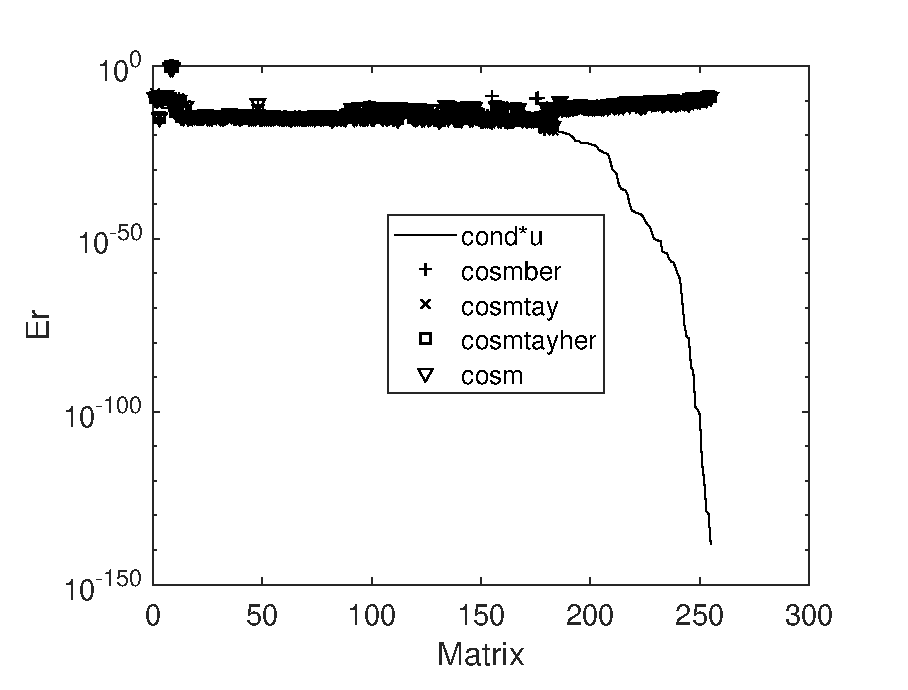
\includegraphics[scale=0.42]{Fig_normwise_9.eps}} %width=40mm
\subfigure[Using formula (\ref{Bernoulli10buena1})]{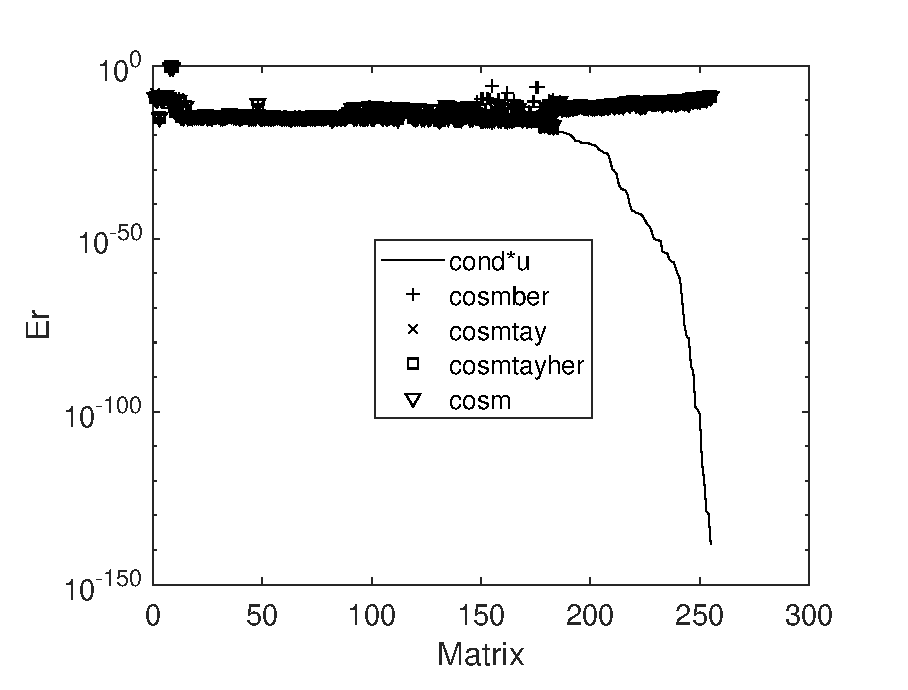
\includegraphics[scale=0.42]{Fig_todas_normwise.eps}}
\caption{Normwise relative errors.} \label{fig:todo}
\end{figure}


\begin{figure}[htbp]
\centering
\subfigure[Using formula (\ref{Bernoulli9buena})]{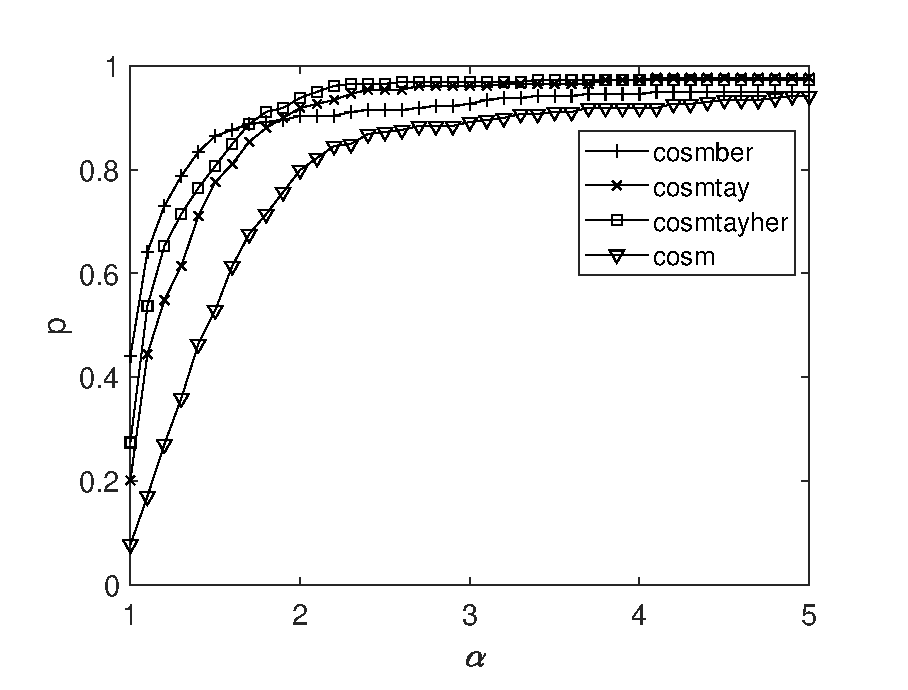
\includegraphics[scale=0.42]{Fig_todas_nprofile_9.eps}} %width=40mm
\subfigure[Using formula (\ref{Bernoulli10buena1})]{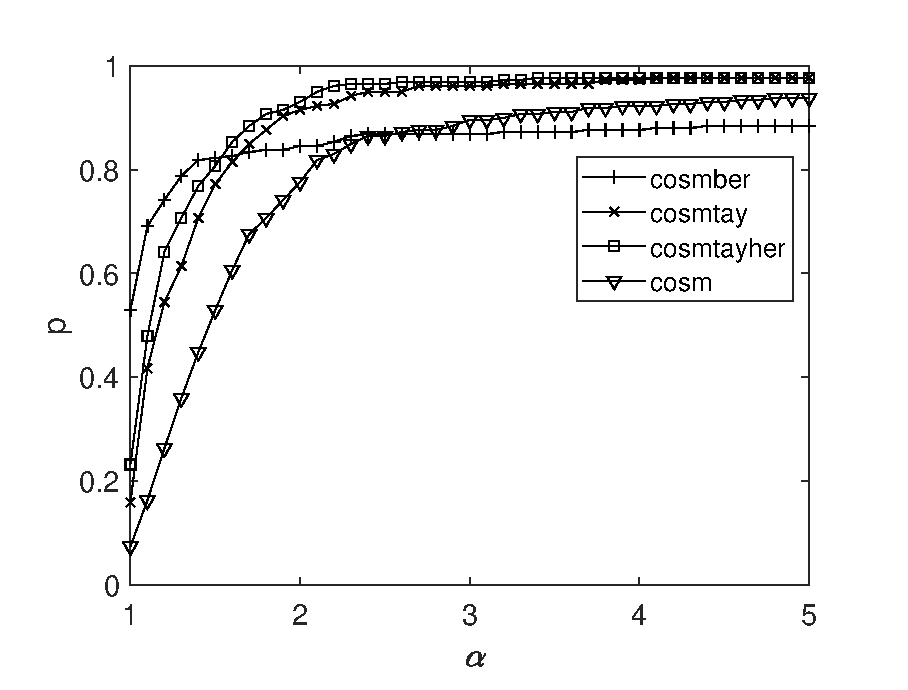
\includegraphics[scale=0.42]{Fig_todas_nprofile.eps}}
\caption{Performance Profile.} \label{fig:todoa}
\end{figure}


\section{Conclusions}\label{section4}

In general, the implementation based on the new Bernoulli series (\ref{Bernoulli10buena1})  is more accurate than (\ref{Bernoulli9buena}), comparing it with the one based on the Taylor series, algorithm  (\texttt{cosmtay}) and Hermite series, algorithm   (\texttt{cosmtayher}), and the one based in Pad\'e  rational approximation, algorithm (\texttt{cosm}).



\bibliographystyle{unsrt}
\bibliography{bib_imm2019}
\end{document}

\newpage

\section{Cada caso por separado}
\subsection{Results with diagonalizable matrices}
Results are given in Tables \ref{tabla_er_comparative_test_1} and \ref{tabla_er_comparative_test_1a}. The rows of each table show the percentage of cases in which the relative errors of \texttt{cosmber} (Bernoulli) are lower, greater or equal than the relative errors of \texttt{cosmtay} (Taylor), \texttt{cosmtayher} (Hermite)  and  \texttt{cosm} (Pad\'e).
Graphics with the Normwise relative errors, see \cite[p. 253]{High08}, using (9) and (10) are given in Figure \ref{fig:caso1}.
Graphics with the Performance Profile, see \cite[p. 254]{High08}, are given in Figure \ref{fig:caso1a}.  Total number of matrix products: \emph{cosmber}: $1279$ \emph{cosmtay}: $933$, \emph{cosmtayher}: $667$,  \emph{cosm}: $1129$.

\begin{figure}[htbp]
\centering
\subfigure[Using formula (\ref{Bernoulli9buena1})]{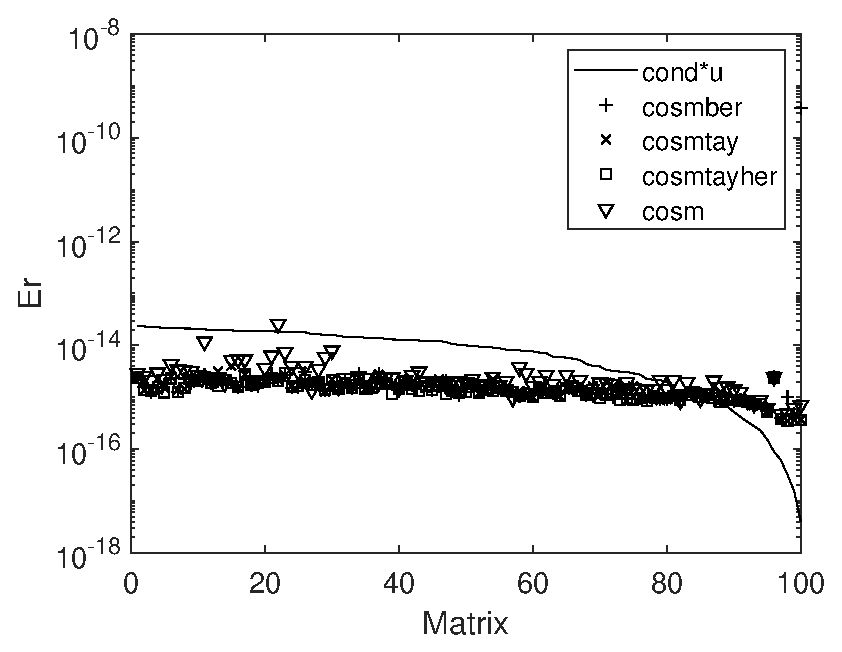
\includegraphics[scale=0.32]{Fig_cos_diag_hadamard_complex_n128_nd256_normwise_cosmber_cosmtay_cosmtayher_cosm_9.eps}} %width=40mm
\subfigure[Using formula (\ref{Bernoulli10buena1a})]{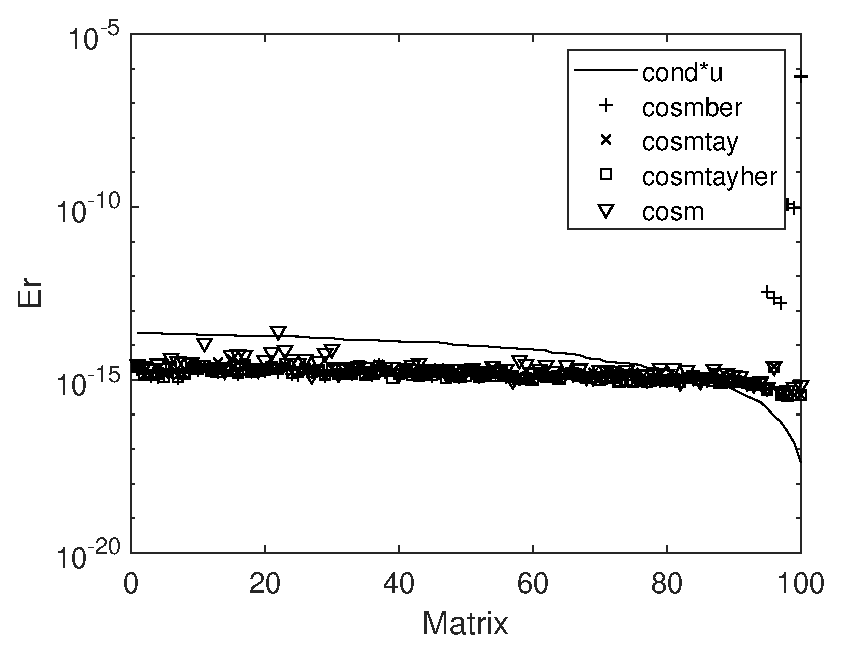
\includegraphics[scale=0.32]{Fig_cos_diag_hadamard_complex_n128_nd256_normwise_cosmber_cosmtay_cosmtayher_cosm.eps}}
\caption{Test 1. Diagonalizable matrices. Normwise relative errors} \label{fig:caso1}
\end{figure}



\begin{figure}[htbp]
\centering
\subfigure[Using formula (\ref{Bernoulli9buena1})]{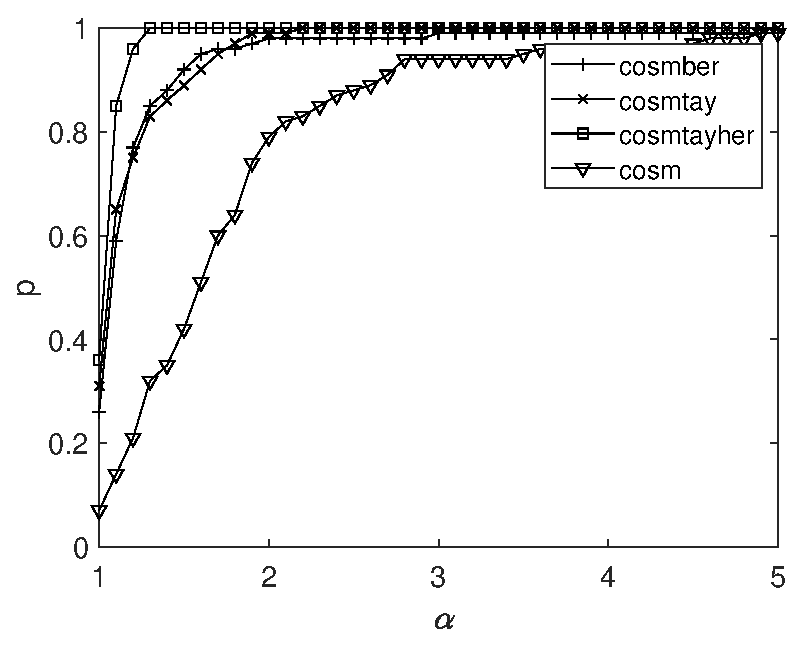
\includegraphics[scale=0.32]{Fig_cos_diag_hadamard_complex_n128_nd256_nprofile__cosmber_cosmtay_cosmtayher_cosm_9.eps}} %width=40mm
\subfigure[Using formula (\ref{Bernoulli10buena1a})]{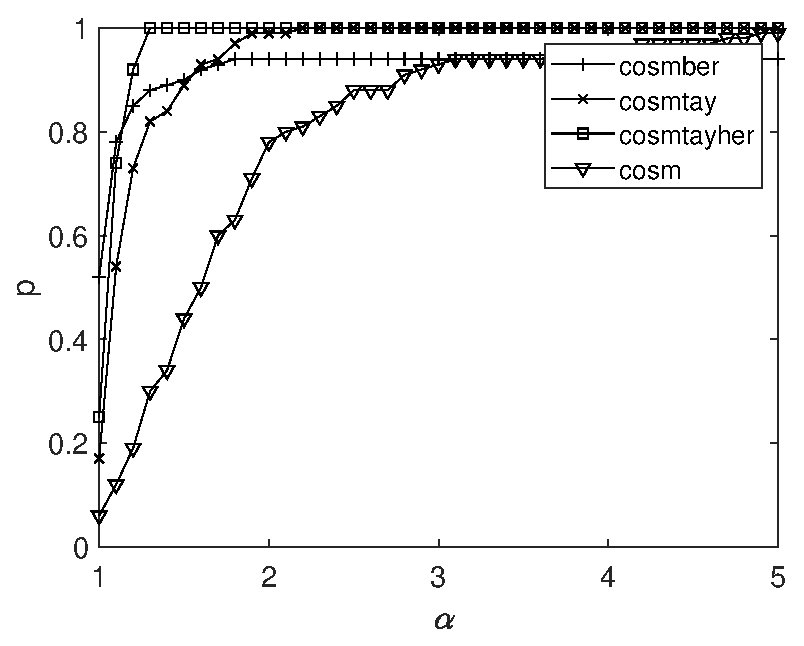
\includegraphics[scale=0.32]{Fig_cos_diag_hadamard_complex_n128_nd256_nprofile__cosmber_cosmtay_cosmtayher_cosm.eps}}
\caption{Test 1. Diagonalizable matrices. Performance Profile.} \label{fig:caso1a}
\end{figure}


\begin{table}[H]\begin{center}
\caption{Using approximation (\ref{Bernoulli9buena1})}
\begin{tabular}{cc}\hline
$E(cosmber)<E(cosmtay)$ & $43.00\%$ \\\hline
$E(cosmber)>E(cosmtay)$ & $57.00\%$ \\\hline
$E(cosmber)=E(cosmtay)$  & $0\%$ \\\hline
$E(cosmber)<E(cosmtayher)$ & $37.00\%$ \\\hline
$E(cosmber)>E(cosmtayher)$ & $63.00\%$ \\\hline
$E(cosmber)=E(cosmtayher)$  & $0\%$ \\\hline
$E(cosmber)<E(cosm)$ & $84.00\%$ \\\hline
$E(cosmber)>E(cosm)$ & $16.00\%$ \\\hline
$E(cosmber)=E(cosm)$  & $0\%$ \\\hline
\end{tabular}
\label{tabla_er_comparative_test_1}
\end{center}
\end{table}

\begin{table}[H]\begin{center}
\caption{Using approximation (\ref{Bernoulli10buena1a})}
\begin{tabular}{cc}\hline
$E(cosmber)<E(cosmtay)$ & $67.00\%$ \\\hline
$E(cosmber)>E(cosmtay)$ & $33.00\%$ \\\hline
$E(cosmber)=E(cosmtay)$  & $0\%$ \\\hline
$E(cosmber)<E(cosmtayher)$ & $60.00\%$ \\\hline
$E(cosmber)>E(cosmtayher)$ & $40.00\%$ \\\hline
$E(cosmber)=E(cosmtayher)$  & $0\%$ \\\hline
$E(cosmber)<E(cosm)$ & $85.00\%$ \\\hline
$E(cosmber)>E(cosm)$ & $15.00\%$ \\\hline
$E(cosmber)=E(cosm)$  & $0\%$ \\\hline
\end{tabular}
\label{tabla_er_comparative_test_1a}
\end{center}
\end{table}

\subsection{Results with non-diagonalizables matrices}
Results are given in Tables \ref{tabla_er_comparative_test_2} and \ref{tabla_er_comparative_test_2a}. Graphics of the Normwise relative errors and the Performance Profile are given in Figures \ref{fig:caso2} and \ref{fig:caso2a}. Total number of matrix products: \emph{cosmber}: $1200$, \emph{cosmtay}: $900$,
\emph{cosmtayher}: $702$,  \emph{cosm}: $1197$.

\begin{table}[H]\begin{center}
\caption{Using approximation (\ref{Bernoulli9buena1})}
\begin{tabular}{cc}\hline
$E(cosmber)<E(cosmtay)$ & $84.00\%$ \\\hline
$E(cosmber)>E(cosmtay)$ & $16.00\%$ \\\hline
$E(cosmber)=E(cosmtay)$  & $0\%$ \\\hline
$E(cosmber)<E(cosmtayher)$ & $85.00\%$ \\\hline
$E(cosmber)>E(cosmtayher)$ & $15.00\%$ \\\hline
$E(cosmber)=E(cosmtayher)$  & $0\%$ \\\hline
$E(cosmber)<E(cosm)$ & $86.00\%$ \\\hline
$E(cosmber)>E(cosm)$ & $14.00\%$ \\\hline
$E(cosmber)=E(cosm)$  & $0\%$ \\\hline
\end{tabular}
\label{tabla_er_comparative_test_2}
\end{center}
\end{table}


\begin{table}[H]\begin{center}
\caption{Using approximation (\ref{Bernoulli10buena1a})}
\begin{tabular}{cc}\hline
$E(cosmber)<E(cosmtay)$ & $84.00\%$ \\\hline
$E(cosmber)>E(cosmtay)$ & $16.00\%$ \\\hline
$E(cosmber)=E(cosmtay)$  & $0\%$ \\\hline
$E(cosmber)<E(cosmtayher)$ & $85.00\%$ \\\hline
$E(cosmber)>E(cosmtayher)$ & $15.00\%$ \\\hline
$E(cosmber)=E(cosmtayher)$  & $0\%$ \\\hline
$E(cosmber)<E(cosm)$ & $86.00\%$ \\\hline
$E(cosmber)>E(cosm)$ & $14.00\%$ \\\hline
$E(cosmber)=E(cosm)$  & $0\%$ \\\hline
\end{tabular}
\label{tabla_er_comparative_test_2a}
\end{center}
\end{table}


\begin{figure}[htbp]
\centering
\subfigure[Using formula (\ref{Bernoulli9buena1})]{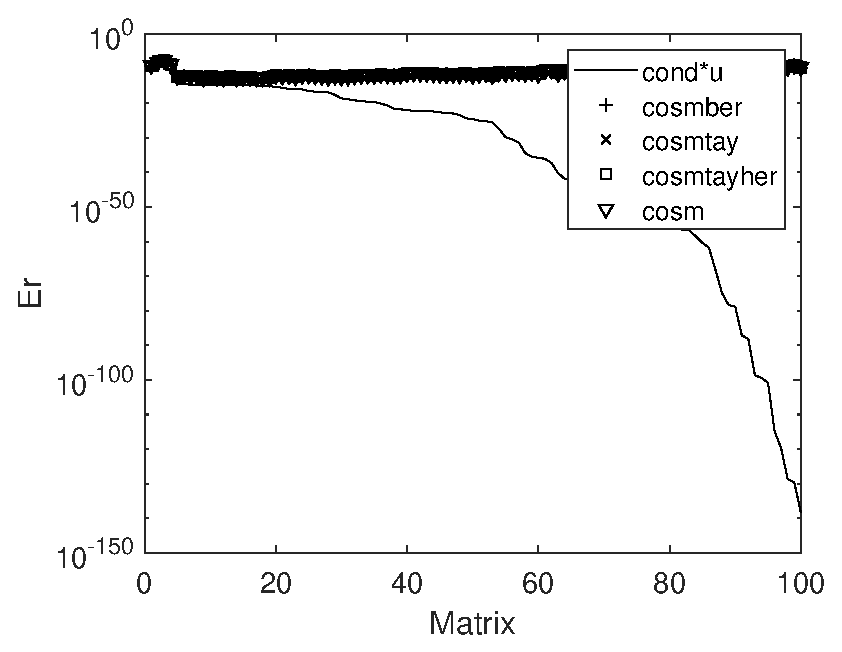
\includegraphics[scale=0.32]{Fig_cos_jordan_random_complex_n128_boundvp10_maxmult5_nd256_normwise_cosmber_cosmtay_cosmtayher_cosm_9.eps}} %width=40mm
\subfigure[Using formula (\ref{Bernoulli10buena1a})]{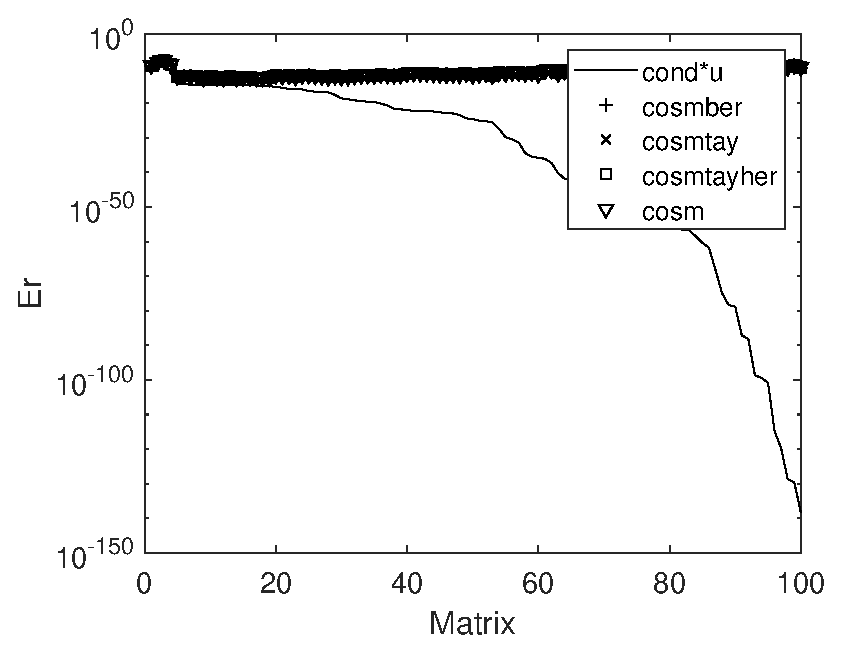
\includegraphics[scale=0.32]{Fig_cos_jordan_random_complex_n128_boundvp10_maxmult5_nd256_normwise_cosmber_cosmtay_cosmtayher_cosm.eps}}
\caption{Test 2. Non-diagonalizable matrices. Normwise relative errors} \label{fig:caso2}
\end{figure}


\begin{figure}[htbp]
\centering
\subfigure[Using formula (\ref{Bernoulli9buena1})]{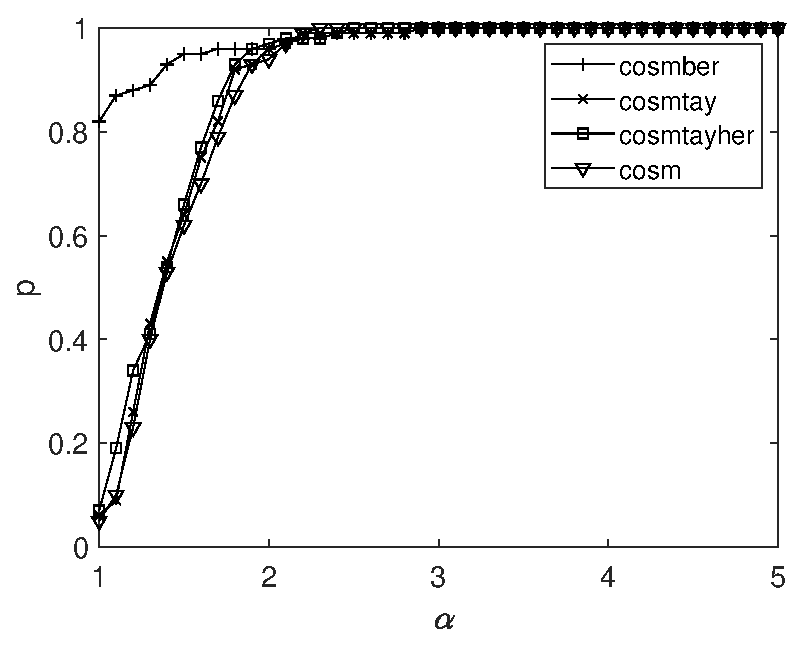
\includegraphics[scale=0.32]{Fig_cos_jordan_random_complex_n128_boundvp10_maxmult5_nd256_nprofile__cosmber_cosmtay_cosmtayher_cosm_9.eps}} %width=40mm
\subfigure[Using formula (\ref{Bernoulli10buena1a})]{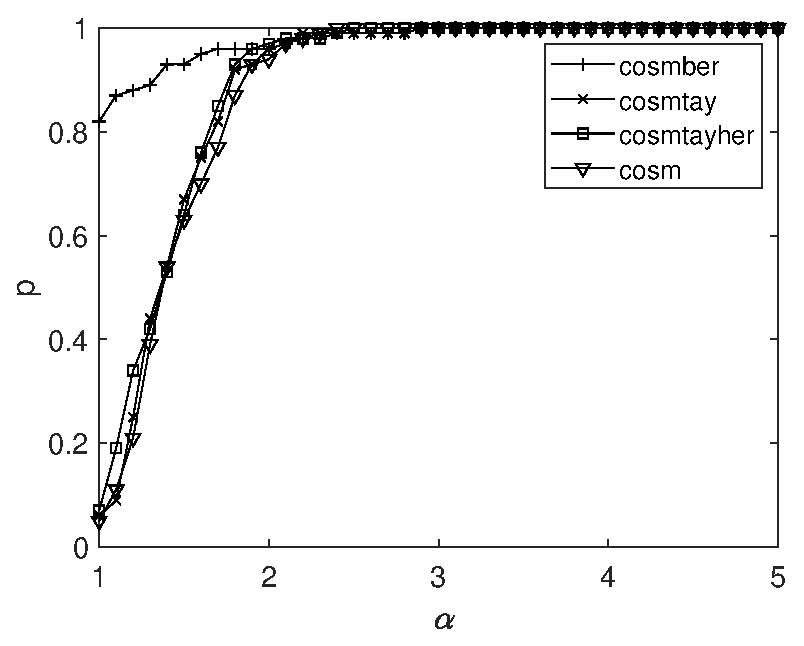
\includegraphics[scale=0.32]{Fig_cos_jordan_random_complex_n128_boundvp10_maxmult5_nd256_nprofile__cosmber_cosmtay_cosmtayher_cosm.eps}}
\caption{Test 2. Non-diagonalizable matrices. Performance Profile.} \label{fig:caso2a}
\end{figure}

\subsection{Results with Matrix Computation Toolbox}
Results are given in Tables \ref{tabla_er_comparative_test_3} and \ref{tabla_er_comparative_test_3a}. Graphics of the Normwise relative errors and the Performance Profile are given in Figures \ref{fig:caso3} and \ref{fig:caso3a}. Total number of matrix products: \emph{cosmber}: $512$ \emph{cosmtay}: $389$, \emph{cosmtayher}: $282$,  \emph{cosm}: $480$.

\begin{table}[H]\begin{center}
\caption{Using approximation (\ref{Bernoulli9buena1})}
\begin{tabular}{cc}\hline
$E(cosmber)<E(cosmtay)$ & $42.86\%$ \\\hline
$E(cosmber)>E(cosmtay)$ & $57.14\%$ \\\hline
$E(cosmber)=E(cosmtay)$  & $0\%$ \\\hline
$E(cosmber)<E(cosmtayher)$ & $28.57\%$ \\\hline
$E(cosmber)>E(cosmtayher)$ & $71.43\%$ \\\hline
$E(cosmber)=E(cosmtayher)$  & $0\%$ \\\hline
$E(cosmber)<E(cosm)$ & $61.90\%$ \\\hline
$E(cosmber)>E(cosm)$ & $38.10\%$ \\\hline
$E(cosmber)=E(cosm)$  & $0\%$ \\\hline
\end{tabular}
\label{tabla_er_comparative_test_3}
\end{center}
\end{table}


\begin{table}[H]\begin{center}
\caption{Using approximation (\ref{Bernoulli10buena1a})}
\begin{tabular}{cc}\hline
$E(cosmber)<E(cosmtay)$ & $35.71\%$ \\\hline
$E(cosmber)>E(cosmtay)$ & $64.29\%$ \\\hline
$E(cosmber)=E(cosmtay)$  & $0\%$ \\\hline
$E(cosmber)<E(cosmtayher)$ & $19.05\%$ \\\hline
$E(cosmber)>E(cosmtayher)$ & $80.95\%$ \\\hline
$E(cosmber)=E(cosmtayher)$  & $0\%$ \\\hline
$E(cosmber)<E(cosm)$ & $50.00\%$ \\\hline
$E(cosmber)>E(cosm)$ & $50.00\%$ \\\hline
$E(cosmber)=E(cosm)$  & $0\%$ \\\hline
\end{tabular}
\label{tabla_er_comparative_test_3a}
\end{center}
\end{table}


\begin{figure}[htbp]
\centering
\subfigure[Using formula (\ref{Bernoulli9buena1})]{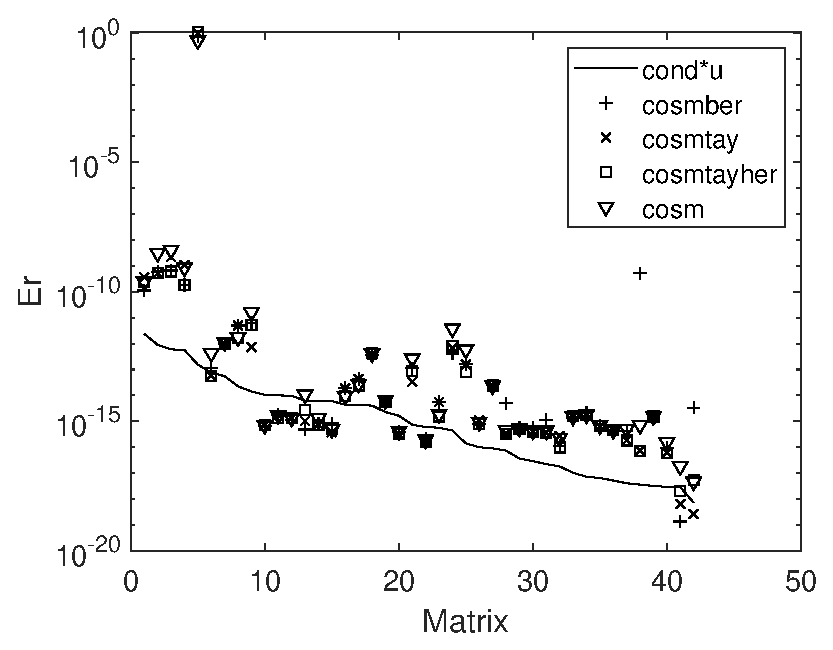
\includegraphics[scale=0.32]{Fig_cos_toolbox_n128_nd256_normwise_cosmber_cosmtay_cosmtayher_cosm_9.eps}} %width=40mm
\subfigure[Using formula (\ref{Bernoulli10buena1a})]{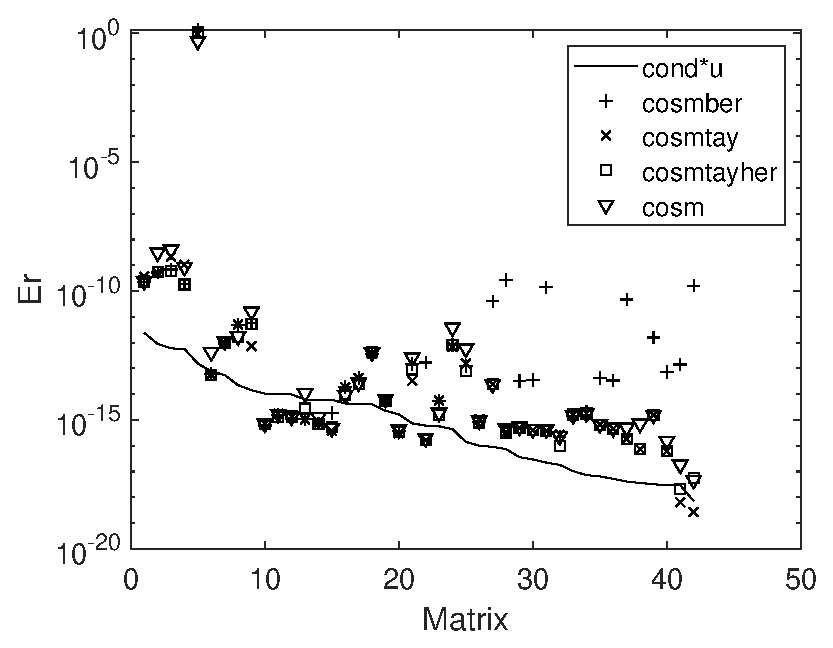
\includegraphics[scale=0.32]{Fig_cos_toolbox_n128_nd256_normwise_cosmber_cosmtay_cosmtayher_cosm.eps}}
\caption{Test 3. Matrix Computation Toolbox. Normwise relative errors} \label{fig:caso3}
\end{figure}


\begin{figure}[htbp]
\centering
\subfigure[Using formula (\ref{Bernoulli9buena1})]{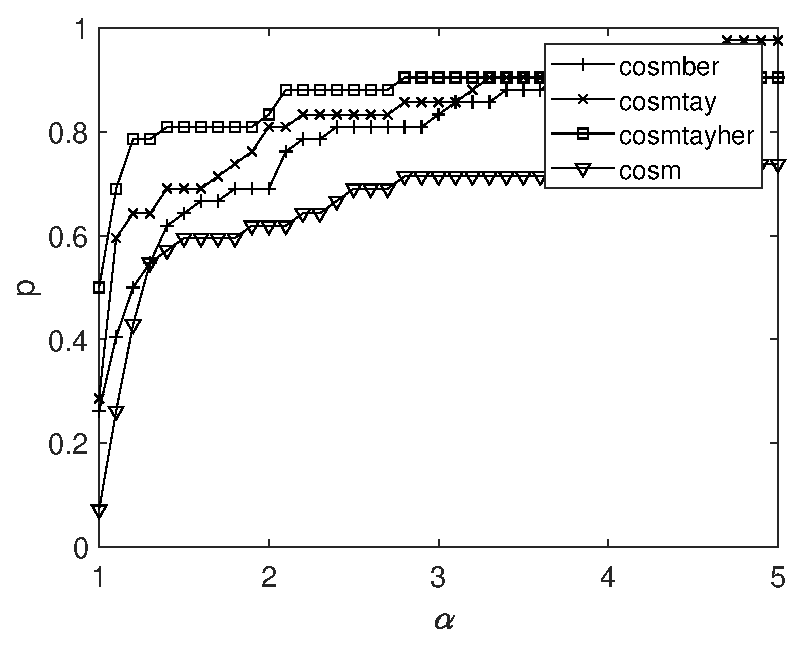
\includegraphics[scale=0.32]{Fig_cos_toolbox_n128_nd256_nprofile__cosmber_cosmtay_cosmtayher_cosm_9.eps}} %width=40mm
\subfigure[Using formula (\ref{Bernoulli10buena1a})]{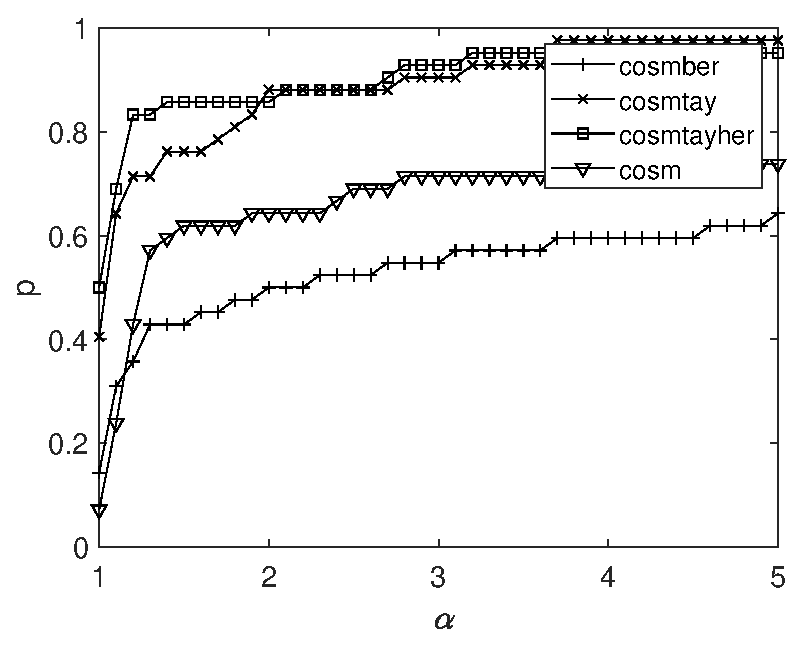
\includegraphics[scale=0.32]{Fig_cos_toolbox_n128_nd256_nprofile__cosmber_cosmtay_cosmtayher_cosm.eps}}
\caption{Test 3. Matrix Computation Toolbox. Performance Profile.} \label{fig:caso3a}
\end{figure}

\subsection{Results with matrices from the Eigtool Matlab package}
Results are given in Tables \ref{tabla_er_comparative_test_4} and \ref{tabla_er_comparative_test_4a}. Graphics of the Normwise relative errors and the Performance Profile are given in Figures \ref{fig:caso4} and \ref{fig:caso4a}. Total number of matrix products: \emph{cosmber}: $211$, \emph{cosmtay}: $169$,
\emph{cosmtayher}: $131$,  \emph{cosm}: $210$.

\begin{table}[H]\begin{center}
\caption{Using approximation (\ref{Bernoulli9buena1})}
\begin{tabular}{cc}\hline
$E(cosmber)<E(cosmtay)$ & $35.29\%$ \\\hline
$E(cosmber)>E(cosmtay)$ & $64.71\%$ \\\hline
$E(cosmber)=E(cosmtay)$  & $0\%$ \\\hline
$E(cosmber)<E(cosmtayher)$ & $17.65\%$ \\\hline
$E(cosmber)>E(cosmtayher)$ & $82.35\%$ \\\hline
$E(cosmber)=E(cosmtayher)$  & $0\%$ \\\hline
$E(cosmber)<E(cosm)$ & $35.29\%$ \\\hline
$E(cosmber)>E(cosm)$ & $64.71\%$ \\\hline
$E(cosmber)=E(cosm)$  & $0\%$ \\\hline
\end{tabular}
\label{tabla_er_comparative_test_4}
\end{center}
\end{table}

\begin{table}[H]\begin{center}
\caption{Using approximation (\ref{Bernoulli10buena1a})}
\begin{tabular}{cc}\hline
$E(cosmber)<E(cosmtay)$ & $16.67\%$ \\\hline
$E(cosmber)>E(cosmtay)$ & $77.78\%$ \\\hline
$E(cosmber)=E(cosmtay)$  & $5.56\%$ \\\hline
$E(cosmber)<E(cosmtayher)$ & $5.56\%$ \\\hline
$E(cosmber)>E(cosmtayher)$ & $88.89\%$ \\\hline
$E(cosmber)=E(cosmtayher)$  & $5.56\%$ \\\hline
$E(cosmber)<E(cosm)$ & $27.78\%$ \\\hline
$E(cosmber)>E(cosm)$ & $66.67\%$ \\\hline
$E(cosmber)=E(cosm)$  & $5.56\%$ \\\hline
\end{tabular}
\label{tabla_er_comparative_test_4a}
\end{center}
\end{table}


\begin{figure}[htbp]
\centering
\subfigure[Using formula (\ref{Bernoulli9buena1})]{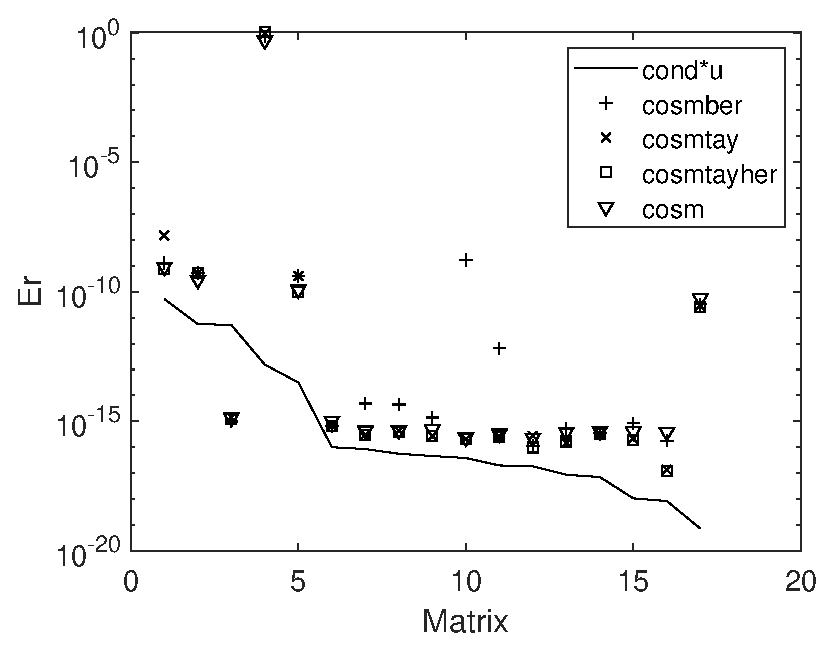
\includegraphics[scale=0.32]{Fig_cos_eigtool_n128_nd256_normwise_cosmber_cosmtay_cosmtayher_cosm_9.eps}} %width=40mm
\subfigure[Using formula (\ref{Bernoulli10buena1a})]{\includegraphics[scale=0.32]{Fig_cos_eigtool_n128_nd256_normwise_cosmber_cosmtay_cosmtayher_cosm.eps}}
\caption{Test 4. Eigtool Matlab package. Normwise relative errors} \label{fig:caso4}
\end{figure}


\begin{figure}[htbp]
\centering
\subfigure[Using formula (\ref{Bernoulli9buena1})]{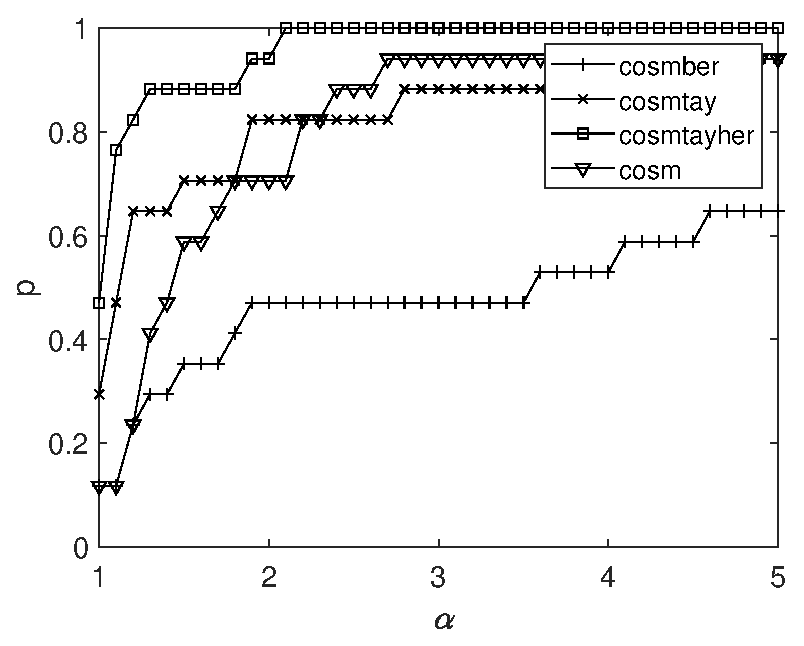
\includegraphics[scale=0.32]{Fig_cos_eigtool_n128_nd256_nprofile__cosmber_cosmtay_cosmtayher_cosm_9.eps}} %width=40mm
\subfigure[Using formula (\ref{Bernoulli10buena1a})]{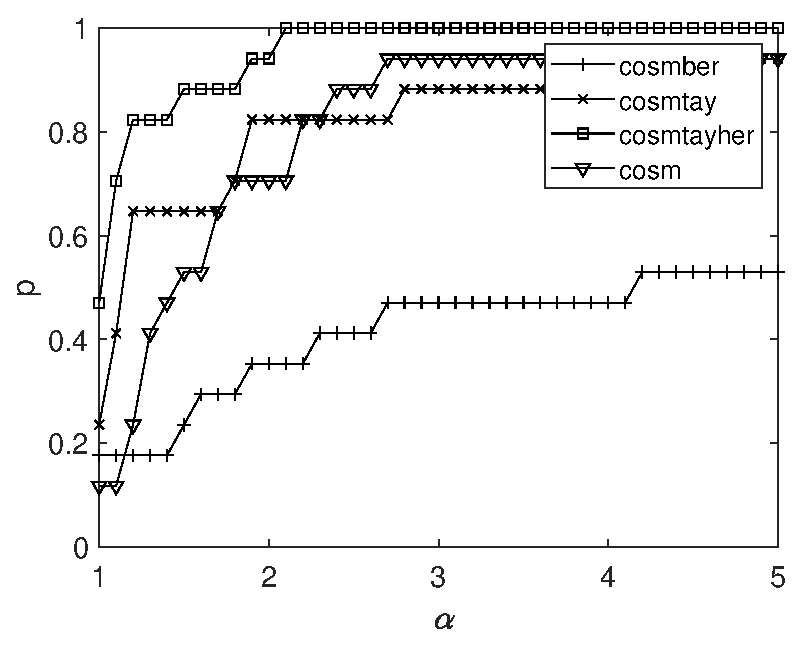
\includegraphics[scale=0.32]{Fig_cos_eigtool_n128_nd256_nprofile__cosmber_cosmtay_cosmtayher_cosm.eps}}
\caption{Test 4. Eigtool Matlab package. Performance Profile.} \label{fig:caso4a}
\end{figure}




